\documentclass[a4paper,14pt]{report}
\usepackage[T2A]{fontenc}
\usepackage[utf8]{inputenc}
\usepackage[english,russian]{babel}
\usepackage{listings}
\usepackage{geometry}
\usepackage{amssymb}
\usepackage{amsmath}
\usepackage[14pt]{extsizes}
\geometry{left=2cm}
\geometry{right=1.5cm}
\geometry{top=1cm}
\geometry{bottom=2cm}
\pagestyle{plain}
\usepackage{pgfplots}
\usepackage{filecontents}
\usepackage{graphicx}
\usepackage{indentfirst}
\DeclareGraphicsExtensions{.png}
\graphicspath{{images/}}
\usetikzlibrary{datavisualization}
\usetikzlibrary{datavisualization.formats.functions}

\usepackage{tocloft}

\renewcommand\cftchapdotsep{\cftdot}
\renewcommand\cftsecdotsep{\cftdot}
\renewcommand{\cftchapleader}{\cftdotfill{\cftchapdotsep}}

\begin{filecontents}{classicEven.dat}
	100 0.0249866
	200 0.1803776
	300 0.6103413
	400 1.452259
	500 2.8890183
	600 5.1179977
	700 8.331629
	800 12.8242005
	900 18.5736184
	1000 27.0825138
\end{filecontents}

\begin{filecontents}{vinogradEven.dat}
	100 0.0170725000
	200 0.1341977500
	300 0.4643969750
	400 1.1203795975
	500 2.2427023597
	600 3.9962032360
	700 6.5615820236
	800 10.1323214024
	900 15.2110748402
	1000 21.6027530840
\end{filecontents}

\begin{filecontents}{optEven.dat}
	100 0.0117449000
	200 0.0942599900
	300 0.3252377990
	400 0.7838837799
	500 1.5808832780
	600 2.8101774278
	700 4.6541242428
	800 7.0837630243
	900 10.6929463024
	1000 15.6942994302
\end{filecontents}


\begin{filecontents}{classicOdd.dat}
	101 0.0239532
	201 0.1823425
	301 0.6155233
	401 1.4677636
	501 2.9109864
	601 5.1334142
	701 8.3448133
	801 13.0947333
	901 19.5909741
	1001 28.395487
\end{filecontents}

\begin{filecontents}{vinogradOdd.dat}
	101 0.0172836000
	201 0.1391932600
	301 0.4704433260
	401 1.1361428326
	501 2.2711334833
	601 4.0243917483
	701 6.5884793748
	801 10.4854465375
	901 16.0785333537
	1001 23.3195016354
\end{filecontents}

\begin{filecontents}{optOdd.dat}
	101 0.0121763000
	201 0.0964552300
	301 0.3295603230
	401 0.7987197323
	501 1.6029470732
	601 2.8370770073
	701 4.6514172007
	801 7.4338798201
	901 11.6243430820
	1001 17.0517238082
\end{filecontents}


% Для листинга кода:
\lstset{ %
language=c++,                 % выбор языка для подсветки
basicstyle=\small\sffamily, % размер и начертание шрифта для подсветки кода
numbers=left,               % где поставить нумерацию строк (слева\справа)
numberstyle=\tiny,           % размер шрифта для номеров строк
stepnumber=1,                   % размер шага между двумя номерами строк
numbersep=5pt,                % как далеко отстоят номера строк от подсвечиваемого кода
showspaces=false,            % показывать или нет пробелы специальными отступами
showstringspaces=false,      % показывать или нет пробелы в строках
showtabs=false,             % показывать или нет табуляцию в строках
frame=single,              % рисовать рамку вокруг кода
tabsize=4,                 % размер табуляции по умолчанию равен 2 пробелам
captionpos=t,              % позиция заголовка вверху [t] или внизу [b]
breaklines=true,           % автоматически переносить строки (да\нет)
breakatwhitespace=false, % переносить строки только если есть пробел
escapeinside={\#*}{*)}   % если нужно добавить комментарии в коде
}

% Для измененных титулов глав:
\usepackage{titlesec, blindtext, color} % подключаем нужные пакеты
\definecolor{gray75}{gray}{0.75} % определяем цвет
\newcommand{\hsp}{\hspace{20pt}} % длина линии в 20pt
% titleformat определяет стиль
\titleformat{\chapter}[hang]{\Huge\bfseries}{\thechapter\hsp\textcolor{gray75}{|}\hsp}{0pt}{\Huge\bfseries}



\begin{document}
\begin{titlepage}
	\centering
	{\scshape\LARGE МГТУ им. Баумана \par}
	\vspace{3cm}
	{\scshape\Large Лабораторная работа №2\par}
	\vspace{0.5cm}
	{\scshape\Large По курсу: "Анализ алгоритмов"\par}
	\vspace{1.5cm}
	{\huge\bfseries Алгоритмы умножения матриц\par}
	\vspace{2cm}
	\Large Работу выполнила: Овчинникова Анастасия, ИУ7-55Б\par
	\vspace{0.5cm}
	\LargeПреподаватели:  Волкова Л.Л., Строганов Ю.В.\par

	\vfill
	\large \textit {Москва, 2019} \par
\end{titlepage}

\tableofcontents

\newpage
\chapter*{Введение}
\addcontentsline{toc}{chapter}{Введение}

Целью данной работы является изучение алгоритмов умножения матриц.

Задачи лабораторной работы:
\begin{enumerate}
	\item реализовать стандартный алгоритм умножения матриц;
	\item реализовать алгоритм умножения матриц Винограда;
	\item реализовать оптимизированный алгоритм умножения матриц Винограда;
	\item дать теоретическую оценку стандартного алгоритма умножения матриц, алгоритма Винограда и оптимизированного алгоритма Винограда;
	\item сравнить время работы перечисленных алгоритмов умножения матриц.
\end{enumerate}


\chapter*{Аналитическая часть}
\addcontentsline{toc}{chapter}{Аналитическая часть}

Матрицей называют математический объект, эквивалентный двумерному массиву. Матрица представляет собой совокупность строк и столбцов, на пересечении которых находятся её элементы. Количество строк и столбцов задает размер матрицы. Будем говорить исключительно о матрицах прямоугольной формы (в частных случаях - квадратной). Для матриц определена операция умножения. Матрица, получаемая в результате операции умножения, называется произведнием матриц.

\section*{Классический алгорим умножения матриц}
\addcontentsline{toc}{section}{Классический алгорим умножения матриц}

Пусть даны две прямоугольные матрицы А и В размерности m на n и n на l соответсвенно:
\[ \begin{bmatrix}
a_{11} & ... & a_{1n} \\
... & ... & ... \\
a_{m1} & ... & a_{mn} \\
\end{bmatrix} \]\\

\[ \begin{bmatrix}
b_{11} & ... & b_{1l} \\
... & ... & ... \\
b_{n1} & ... & b_{nl} \\
\end{bmatrix} \]\\

Тогда матрица C размерностью m на l:

\[ \begin{bmatrix}
c_{11} & ... & c_{1l} \\
... & ... & ... \\
c_{m1} & ... & c_{ml} \\
\end{bmatrix} \]\\

в которой:

$c_{ij} = \sum\limits_{r=1}^n a_{ir}\cdot b_{rj}  (i = 0, 1, ..., m - 1; j = 0, 1, ..., l - 1)$

называется произведением матриц A и B.

\section*{Алгоритм Винограда}
\addcontentsline{toc}{section}{Алгоритм Винограда}

Если посмотреть на результат умножения двух матриц, то видно, что каждый элемент в нем представляет собой скалярное произведение соответствующих строки и столбца исходных матриц. Можно заметить также, что такое умножение допускает предварительную обработку, позволяющую часть работы выполнить заранее.

Алгоритм Винограда считается более эффективным благодаря сокращению количества операций умножения.

Рассмотрим два вектора $V = (v1, v2, v3, v4)$ и $W = (w1, w2, w3, w4)$. Их скалярное произведение равно:

$ V \cdot W=v_1 \cdot w_1 + v_2 \cdot w_2 + v_3 \cdot w_3 + v_4 \cdot w_4$ \\

Это равенство можно переписать в виде: \\
$V \cdot W=(v_1 + w_2) \cdot (v_2 + w_1) + (v_3 + w_4) \cdot (v_4 + w_3) - v_1 \cdot v_2 - v_3 \cdot v_4 - w_1 \cdot w_2 - w_3 \cdot w_4$\\

Менее очевидно, что выражение в правой части последнего равенства допускает предварительную обработку: его части можно вычислить заранее и запомнить для каждой строки первой матрицы и для каждого столбца второй.
Это означает, что над предварительно обработанными элементами нам придется выполнять лишь первые два умножения и последующие пять сложений, а также дополнительно два сложения.

\section*{Улучшенный алгоритм Винограда}
\addcontentsline{toc}{section}{Улучшенный алгоритм Винограда}

Улучшить алгоритм Винограда можно следующим образом.

\begin{enumerate}
	\item Добавление дополнительного буфера для уменшения количества обращений к результирующей матрице.
	\item Уменьшение количества операций умножения при заполнении дополнительных массивов, необходимых для работы алгоритма: mulH и mulV (подробнее см. далее).
	\item Замена операций типа $x = x + y$ на операции $x += y$.
	\item Избавиться от делений в заголовках циклов.
\end{enumerate}

\section*{Модель вычислений}
\addcontentsline{toc}{section}{Модель вычислений}

Трудоемкость алгоритма измеряется в количестве операций, которые необходимо выполнить.

Введем модель вычислений, используемую при оценке трудоемкости алгоритмов.

\begin{enumerate}
	\item Базовые операции трудоемкости 1: +, -, *, /, =, ==, <=, >=, !=, >, <, +=, -=, |=, *=, проход по адресу.
	\item Трудоемкость цикла вычисляется по формуле $f = 2 + N(2 + f_{body})$, где $N$ - число повтрорений цикла, $f_{body}$ - трудоемкость тела цикла.
	\item Трудоемкость условного перехода равна 0, стоимость вычисления условия остается.
	\item Вызов метода объекта класса имеет трудоемкость 1.
	\item Объявление переменной/массива/структуры без определения имеет трудоемкость 0.\
	\item Условный оператор без условий внутри имеет трудоемкость 0.
	\item Логические операции имеют трудоемкость 1.
\end{enumerate}

\section*{Вывод}
\addcontentsline{toc}{section}{Вывод}
В данном разделе были рассмотрены идеи классического алгоритма умножения матриц, алгорима Винограда и улучшенного алгоритма Винограда. Более подробно эти алгоритмы (в т.ч. их схемы) будут рассмотрены в следующих разделах.

\chapter*{Конструкторская часть}
\addcontentsline{toc}{chapter}{Конструкторская часть}

\section*{Требования к программе}
\addcontentsline{toc}{section}{Требования к программе}

\textbf{Требования к вводу:}\\
На вход программе подаются две матрицы и их размерности.\\

\textbf{Требования к программе:}\\
Корректное умножение двух матриц.\\

%Программа представляет собой консольное приложение с меню для выбора пользователем необходимого действия.
%Меню содержит следующие пункты:
%\begin{itemize}
%	\item "1 - умножение случайной матрицы с помощью классического алгоритма умножения матриц";
%	\item "2 - умножение случайной матрицы с помощью классического алгоритма Винограда";
%	\item "3 - умножение случайной матрицы с помощью классического оптимизированного алгоритма Винограда";
%	\item "4 - временной анализ";
%	\item "5 - тесты".
%\end{itemize}

%Для выбора соответствующих пунктов меню пользователь вводит соответствующую цифру (1-5). При вводе любого другого символа программа должна корректно завершаться. Для пунктов 1 - 3 программа просит пользователя ввести желаемую размерность матрицы. Затем она генерирует случайную матрицу указанной размерности с помощью втроенной функции rand().

%Далее в данном разделе будут рассмотрены схемы классического алгорима умножения матриц, алгорима Винограда и оптимизированного алгорима Винограда.

\section*{Схемы алгоритмов}
\addcontentsline{toc}{section}{Схемы алгоритмов}

На рисунке 1 представлена схема классического алгорима умножения матриц. На рисунке 2 представлена схема алгорима Винограда. На рисунке 3 представлена схема оптимизированного алгорима Винограда. В схемах используются обозначения, которые были введены при рассмотрении алгоритмов умножения матриц в предыдущем разделе.

\begin{figure}
\center{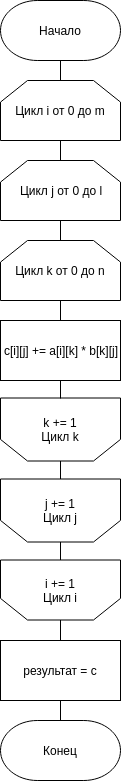
\includegraphics[height=20cm]{classicMult.png}}
\caption{Схема классического алгорима умножения матриц}
\label{fig:image}
\end{figure}

\begin{figure}
\center{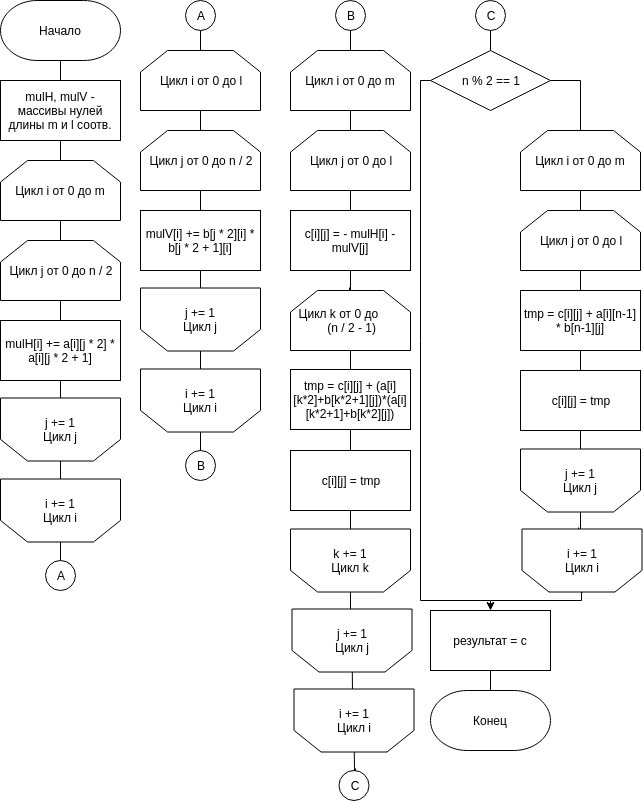
\includegraphics[height=20cm]{vinograd.png}}
\caption{Схема алгоритма Винограда}
\label{fig:image}
\end{figure}

\begin{figure}
\center{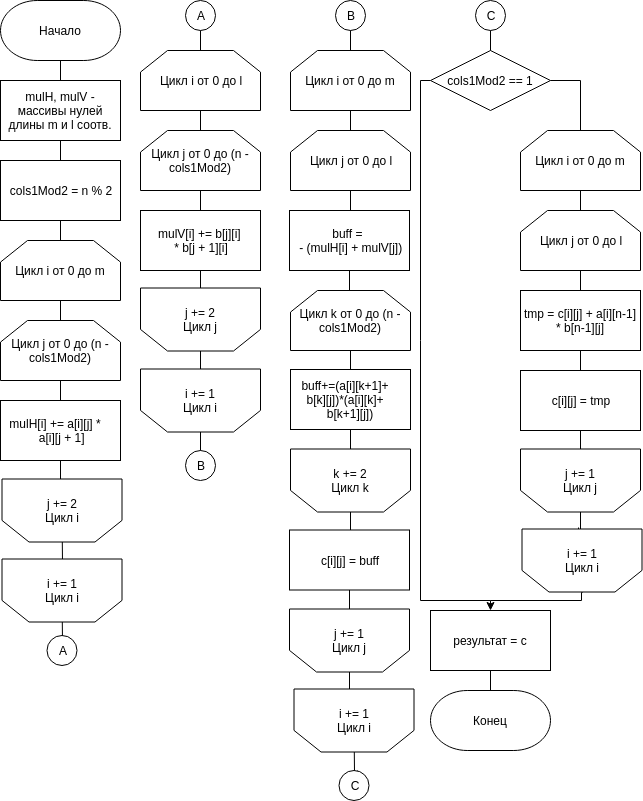
\includegraphics[height=20cm]{optVinograd.png}}
\caption{Схема оптимизированного алгорима Винограда}
\label{fig:image}
\end{figure}


\chapter*{Технологическая часть}
\addcontentsline{toc}{chapter}{Технологическая часть}

\section*{Выбор языка программирования}
\addcontentsline{toc}{section}{Выбор языка программирования}

В качестве языка программирования для реализации программы был выбран язык C++ и фреймворк Qt, потому что:
\begin{itemize}
	\item язык C++ имеет высокую вычислительную производительность;
	\item язык C++ поддерживает различные стили программирования;
	\item в Qt существует удобный инструмент для тестирования - QtTest - который позволяет собирать тесты в группы, собирать результаты выполнения тестов, а также уменьшить дублирование кода при схожих объектах тестирования.
\end{itemize}

Для замеров времени использовалась функция clock() модуля ctime. Эта функция возвращает количество временных тактов, прошедших с начала запуска программы. С помощью макроса CLOCKS\_PER\_SEC можно узнать количество пройденных тактов за 1 секунду.

\section*{Сведения о модулях программы}
\addcontentsline{toc}{section}{Сведения о модулях программы}

Программа состоит из следующих файлов:
\begin{itemize}
	\item mymatrix.h, mymatrix.cpp - заголовочный файл и файл, в котором расположена реализация алгоритмов сортировки;
	\item main.cpp - главный файл программы, в котором расположена реализация меню;
	\item testmymatrix.h, testmymatrix.cpp - файл и заголовочный файл, в котором расположена реализация тестов.
\end{itemize}


\section*{Листинги кода алгоритмов}
\addcontentsline{toc}{section}{Листинги кода алгоритмов}

Код классического алгоритма умножения матриц представлен в листинге 1. Код алгоритма Винограда представлен в листинге 2. Код оптимизированного алгоритма Винограда представлен в листинге 3.

\begin{lstlisting}[label=some-code,caption=Классический алгоритм умножения матриц]
MyMatrix MyMatrix::multiply(const MyMatrix &m)
{
    if (mColumns != m.mRows)
        throw std::logic_error("Attempt to multiply matrices of different dimensions.");

    MyMatrix result(mRows, m.mColumns, 0);

    for (int i = 0; i < mRows; ++i)
        for (int j = 0; j < m.mColumns; ++j)
            for (int k = 0; k < mColumns; ++k)
            {
                int resNum = result.at(i, j) + this->at(i, k) * m.at(k, j);
                result.set(i, j, resNum);
            }
    return result;
}
\end{lstlisting}

\begin{lstlisting}[label=some-code,caption=Алгоритм Винограда]
MyMatrix MyMatrix::multiplyVinograd(const MyMatrix &m)
{
    if (mColumns != m.mRows)
        throw std::logic_error("Attempt to multiply matrices of different dimensions.");

    MyMatrix result(mRows, m.mColumns, 0);

    int* mulH = new int[result.mRows];
    int* mulV = new int[result.mColumns];

    for (int i = 0; i < result.mRows; ++i)
        mulH[i] = 0;
    for (int i = 0; i < result.mColumns; ++i)
        mulV[i] = 0;

    for (int i = 0; i < result.mRows; ++i)
        for (int j = 0; j < m.mRows / 2; ++j)
            mulH[i] += this->at(i, j * 2) * this->at(i, j * 2 + 1);

    for (int i = 0; i < result.mColumns; ++i)
        for (int j = 0; j < m.mRows / 2; ++j)
            mulV[i] += m.at(2 * j, i) * m.at(j * 2 + 1, i);

    for (int i = 0; i < result.mRows; ++i)
        for (int j = 0; j < result.mColumns; ++j)
        {
            result.set(i, j, - mulH[i] - mulV[j]);
            for (int k = 0; k < m.mRows / 2; ++k)
            {
                int newRes = result.at(i, j) +
                             (this->at(i, 2 * k) + m.at(2 * k + 1, j)) *
                             (this->at(i, 2 * k + 1) + m.at(2 * k, j));
                result.set(i, j, newRes);
            }
        }

    if (mColumns % 2)
    {
        for (int i = 0; i < mRows; ++i)
            for (int j = 0; j < m.mColumns; ++j)
            {
                int newRes = result.at(i, j) +
                             this->at(i, mColumns - 1) *
                             m.at(mColumns - 1, j);
                result.set(i, j, newRes);
            }
    }
    delete [] mulH;
    delete [] mulV;
    return result;
}
\end{lstlisting}

\begin{lstlisting}[label=some-code,caption=Оптимизированный алгорим Винограда]
MyMatrix MyMatrix::multiplyVinogradOptimized(const MyMatrix &m)
{
    if (mColumns != m.mRows)
        throw std::logic_error("Attempt to multiply matrices of different dimensions.");

    MyMatrix result(mRows, m.mColumns, 0);

    int* mulH = new int[result.mRows];
    int* mulV = new int[result.mColumns];

    for (int i = 0; i < result.mRows; ++i)
        mulH[i] = 0;
    for (int i = 0; i < result.mColumns; ++i)
        mulV[i] = 0;

    int cols1Mod2 = mColumns % 2;

    for (int i = 0; i < mRows; ++i)
        for (int j = 0; j < (mColumns - cols1Mod2); j += 2)
            mulH[i] += this->at(i, j) * this->at(i, j + 1);

    for (int i = 0; i < m.mColumns; ++i)
        for (int j = 0; j < (m.mRows - cols1Mod2); j += 2)
            mulV[i] += m.at(j, i) * m.at(j + 1, i);

    for (int i = 0; i < mRows; ++i)
        for (int j = 0; j < m.mColumns; ++j)
        {
            int buff = -(mulH[i] + mulV[j]);
            for (int k = 0; k < (mColumns - cols1Mod2); k += 2)
                buff += (this->at(i, k + 1) + m.at(k, j)) *
                        (this->at(i, k) + m.at(k + 1, j));
            result.set(i, j, buff);
        }

    if (cols1Mod2)
    {
        for (int i = 0; i < result.mRows; ++i)
            for (int j = 0; j < result.mColumns; ++j)
            {
                int newRes = result.at(i, j) +
                             this->at(i, mColumns - 1) *
                             m.at(mColumns - 1, j);
                result.set(i, j, newRes);
            }
    }
    delete [] mulH;
    delete [] mulV;
    return result;
}
\end{lstlisting}


\section*{Расчет трудоемкости}
\addcontentsline{toc}{section}{Расчет трудоемкости}

\subsection*{Классический алгорим умножения матриц}
\addcontentsline{toc}{section}{Классический алгорим умножения матриц}

Рассмотрим трудоемкость классического алгоритма умножения матриц.\\

$f = 2 + m(2 + 2 + l(2 + 2 + n(2 + 7))) = 2 + m(4 + l(4 + 9n)) = 2 + m(4 + 4l + 9ln) = 2 + 4m + 4lm + 9lmn$ \\

\subsection*{Алгоритм Винограда}
\addcontentsline{toc}{section}{Алгоритм Винограда}

Рассмотрим трудоемкость алгоритма Винограда.

%1 цикл:

%$f_{1} = 2 + m(2 + 2) = 2 + 4m$

%2 цикл:

%$f_{2} = 2 + 4l$

1 цикл:

$f_{1} = 2 + m(4 + 10 \frac{n}{2})) = 2 + m(4 + 5n) = 2 + 4m + 5nm$

2 цикл:

$f_{2} = 2 + l(4 + 10\frac{n}{2}) = 2 + l(4 + 5n) = 2 + 4l + 5ln$

3 цикл:

$f_{3} = 2 + m(4 + l(2 + 5 + 2 + \frac{n}{2}(2 + 15))) = 2 + m(4 + l(9 + 17\frac{n}{2})) = 2 + m(4 + 9l + \frac{17}{2}ln) = 2 + 4m + 9lm + \frac{17}{2}lmn$

Условный переход:

$f_{c} = \begin{bmatrix}
2, \text{если n mod 2 == 0} \\
2 + 4m + 10lm, \text{иначе} \\
\end{bmatrix}$

Итого:

$f = f_{1} + f_{2} + f_{3} + f_{c} = 6 + 8m + 5nm + 4l + 5ln + 9lm + \frac{17}{2}lmn + \begin{bmatrix}
2, \text{если n mod 2 == 0} \\
2 + 4m + 10lm, \text{иначе} \\
\end{bmatrix}$

\subsection*{Оптимизированный алгоритм Винограда}
\addcontentsline{toc}{section}{Оптимизированный алгоритм Винограда}

Рассмотрим трудоемкость оптимизированного алгоритма Винограда.\\

1 цикл:

$f_{1} = 2 + m(5 + 4n) = 2 + 5m + 4mn$

2 цикл:

$f_{2} = 2 + 5l + 4 ln$

3 цикл:

$f_{3} = 2 + 4m + 7lm + \frac{13}{2}lmn$

Условный переход:

$f_{c} = \begin{bmatrix}
1, \text{если n mod 2 == 0} \\
2 + 4m + 9lm, \text{иначе} \\
\end{bmatrix}$

Итого:

$f = f_{1} + f_{2} + f_{3} + f_{c} = 7 + 8m + 4mn + 4l + 4ln + 9lm + \frac{13}{2}lmn$

\section*{Тесты}
\addcontentsline{toc}{section}{Тесты}

Тестирование проводилось с помощью модуля QtTest. Для этого был написан класс TestMyMatrix. Сначала каждый алгоритм умножения матриц тестировался по отдельности на заранее заготовленном наборе тестовых данных.
После этого генерировались пары случайных квадратных матриц целых чисел в диапазоне от -50 до 50 размером от 0 до 200 с шагом 5 (для каждой размерности матрицы генерировалось 10 случайных матриц). Проводилоь умножение этих пар матриц с помощью классического алгоритма умножения матриц, алгорима Винограда и оптимизированного алгорима Винограда и сравнивались результаты работы этих трех алгоритмов. Затем генерировались пары случайных прямоугольных матриц целых чисел в диапазоне от -50 до 50 размером от 0 до 200 с шагом 5 (для каждой размерности матрицы генерировалось 10 случайных матриц). Проводилась умножение этих пар матриц с помощью классического алгоритма умножения матриц, алгорима Винограда и оптимизированного алгорима Винограда и сравнивались результаты работы этих трех алгоритмов.

Все написанные тесты были пройдены.

Использованный набор тестовых данных приведен в таблице 1.

\begin{table}[h]
	\caption{Набор тестовых данных}
	%\begin{center}
		\begin{tabular}{|c | c | c |}
	 	\hline
		Матрица 1 & Матрица 2 & Ожидаемый результат \\ [0.5ex]
	 	\hline\hline
		[0] & [0] & [0] \\
		\hline
		[0] & [1] & [0] \\
		\hline
		[1] & [1] & [1] \\
		\hline
		[2] & [2] & [4] \\
		\hline
		$\begin{bmatrix}
		1 & 1 \\
		1 & 1 \\
		\end{bmatrix}$ &
		$\begin{bmatrix}
		1 & 1 \\
		1 & 1 \\
		\end{bmatrix}$ &
		$\begin{bmatrix}
		2 & 2 \\
		2 & 2 \\
		\end{bmatrix}$ \\
		\hline
		$\begin{bmatrix}
		2 & 2 \\
		2 & 2 \\
		\end{bmatrix}$ &
		$\begin{bmatrix}
		2 & 2 \\
		2 & 2 \\
		\end{bmatrix}$ &
		$\begin{bmatrix}
		8 & 8 \\
		8 & 8 \\
		\end{bmatrix}$ \\
		\hline

		$\begin{bmatrix}
		0 & 0 \\
		0 & 0 \\
		\end{bmatrix}$ &
		$\begin{bmatrix}
		0 & 0 \\
		0 & 0 \\
		\end{bmatrix}$ &
		$\begin{bmatrix}
		0 & 0 \\
		0 & 0 \\
		\end{bmatrix}$ \\
		\hline

		$\begin{bmatrix}
		0 & 0 \\
		0 & 0 \\
		\end{bmatrix}$ &
		$\begin{bmatrix}
		1 & 1 \\
		1 & 1 \\
		\end{bmatrix}$ &
		$\begin{bmatrix}
		0 & 0 \\
		0 & 0 \\
		\end{bmatrix}$ \\
		\hline

		$\begin{bmatrix}
		1 & 2 \\
		3 & 4 \\
		\end{bmatrix}$ &
		$\begin{bmatrix}
		1 & 1 \\
		1 & 1 \\
		\end{bmatrix}$ &
		$\begin{bmatrix}
		3 & 3 \\
		7 & 7 \\
		\end{bmatrix}$ \\
		\hline

		$\begin{bmatrix}
		1 & 1 \\
		1 & 1 \\
		\end{bmatrix}$ &
		$\begin{bmatrix}
		1 & 2 \\
		3 & 4 \\
		\end{bmatrix}$ &
		$\begin{bmatrix}
		4 & 6 \\
		4 & 6 \\
		\end{bmatrix}$ \\
		\hline

		$\begin{bmatrix}
		1 & 2 \\
		3 & 4 \\
		\end{bmatrix}$ &
		$\begin{bmatrix}
		1 & 2 \\
		3 & 4 \\
		\end{bmatrix}$ &
		$\begin{bmatrix}
		7 & 10 \\
		15 & 22 \\
		\end{bmatrix}$ \\
		\hline

		$\begin{bmatrix}
		1 \\
		1 \\
		\end{bmatrix}$ &
		$\begin{bmatrix}
		1 & 1 \\
		\end{bmatrix}$ &
		$\begin{bmatrix}
		1 & 1 \\
		1 & 1 \\
		\end{bmatrix}$ \\
		\hline

		$\begin{bmatrix}
		1 & 1\\
		\end{bmatrix}$ &
		$\begin{bmatrix}
		1 \\
		1 \\
		\end{bmatrix}$ &
		$\begin{bmatrix}
		1 & 1 \\
		1 & 1 \\
		\end{bmatrix}$ \\
		\hline

		$\begin{bmatrix}
		1 & 2 \\
		3 & 4 \\
		5 & 6 \\
		\end{bmatrix}$ &
		$\begin{bmatrix}
		6 & 5 & 4 \\
		3 & 2 & 1\\
		\end{bmatrix}$ &
		$\begin{bmatrix}
		12 & 9 & 6 \\
		30 & 23 & 16 \\
		48 & 37 & 26 \\
		\end{bmatrix}$ \\
		\hline

		$\begin{bmatrix}
		1 & 4 & 8 \\
		16 & 32 & 64 \\
		\end{bmatrix}$ &
		$\begin{bmatrix}
		1 & 3 \\
		9 & 27 \\
		81 & 243 \\
		\end{bmatrix}$ &
		$\begin{bmatrix}
		685 & 2055 \\
		5488 & 16464 \\
		\end{bmatrix}$ \\
		\hline

		$\begin{bmatrix}
		1 & 4 & 1 \\
		5 & 9 & 2 \\
		6 & 5 & 3 \\
		5 & 8 & 9 \\
		\end{bmatrix}$ &
		$\begin{bmatrix}
		7 & 9 & 3 & 2 \\
		3 & 8 & 4 & 6 \\
		2 & 6 & 4 & 3 \\
		\end{bmatrix}$ &
		$\begin{bmatrix}
		21 & 47 & 23 & 29 \\
		66 & 129 & 59 & 70 \\
		63 & 112 & 50 & 51 \\
		77 & 163 & 83 & 85 \\
		\end{bmatrix}$ \\
		\hline

		\end{tabular}
	%\end{center}
\end{table}

\chapter*{Исследовательская часть}
\addcontentsline{toc}{chapter}{Исследовательская часть}

\section*{Постановка эксперимента}
\addcontentsline{toc}{section}{Постановка эксперимента}

В рамках данной работы были проведены следующие эксперименты.

\begin{enumerate}
	\item Замеры времени работы классического алгорима умножения матриц для квадратных матриц размерностей от 100 x 100 до 1000 x 1000 с шагом 100.
	\item Замеры времени работы алгорима Винограда для квадратных матриц размерностей от 100 x 100 до 1000 x 1000 с шагом 100.
	\item Замеры времени работы оптимизированного алгорима Винограда для квадратных матриц размерностей от 100 x 100 до 1000 x 1000 с шагом 100.
	\item Замеры времени работы классического алгорима умножения матриц для квадратных матриц размерностей от 101 x 101 до 1001 x 1001 с шагом 100.
	\item Замеры времени работы алгорима Винограда для квадратных матриц размерностей от 101 x 101 до 1001 x 1001 с шагом 100.
	\item Замеры времени работы оптимизированного алгорима Винограда для квадратных матриц размерностей от 101 x 101 до 1001 x 1001 с шагом 100.
\end{enumerate}

В рамках каждого эксперимента для матриц каждой размерности проводилось по 10 замеров, и вычислялось среднее время работы конкретного алгоритма на матрицах данной размерности.

Измерения проводились на компьютере HP Pavilion Notebook на базе Intel Core i5-7200U, 2.50 Гц с 6 Гб оперативной памяти под управлением операционной системы Linux Mint.

\section*{Сравнительный анализ на материале экспериментальных данных}
\addcontentsline{toc}{section}{Сравнительный анализ на материале экспериментальных данных}

В таблице 2 представлены результаты замеров времени работы классического алгоритма умножения матрц (Классич.), алгоритма Винограда (Виноград) и оптимизированного алгорима Винограда (Опт. Виноград) на квадратных матрицах четного размера.

\begin{table}
	\caption{Результаты замеров времени для матриц четного размера}
	%\begin{center}
		\begin{tabular}{|c | c | c | c |}
	 	\hline
		Размерность & Классич., с & Виноград, с & Опт. Виноград, с \\ [0.5ex]
	 	\hline\hline
		100 & 0.0249866 & 0.0170725 & 0.0117449 \\ \hline
		200 & 0.1803776 & 0.13419775 & 0.09425999 \\ \hline
		300 & 0.6103413 & 0.464396975 & 0.325237799 \\ \hline
		400 & 1.452259 & 1.1203795975 & 0.7838837799 \\ \hline
		500 & 2.8890183 & 2.2427023597 & 1.580883278 \\ \hline
		600 & 5.1179977 & 3.996203236 & 2.8101774278 \\ \hline
		700 & 8.331629 & 6.5615820236 & 4.6541242428 \\ \hline
		800 & 12.8242005 & 10.1323214024 & 7.0837630243 \\ \hline
		900 & 18.5736184 & 15.2110748402 & 10.6929463024 \\ \hline
		1000 & 27.0825138 & 21.602753084 & 15.6942994302 \\ \hline
		\end{tabular}
	%\end{center}
\end{table}

\newpage
Данные из таблицы 2 изображены на рисунке 4. Условные обозначения:

\begin{itemize}
	\item classicEven - время работы классического алгоритма умножения матриц на квадратных матрицах четного размера в секундах;
		\item vinogradEven - время работы алгорима Винограда на квадратных матрицах четного размера в секундах;
			\item optEven - время работы оптимизированного алгорима Винограда на квадратных матрицах четного размера в секундах.
\end{itemize}

\begin{figure}[!h]
	\center{
	\begin{tikzpicture}
	\begin{axis}[
	    	axis lines = left,
	    	xlabel = {размерность},
	    	ylabel = {время, с},
		legend pos=north west,
		ymajorgrids=true
	]
	\addplot[color=blue, mark=square] table[x index=0, y index=1] {classicEven.dat};
	\addplot[color=green, mark=square] table[x index=0, y index=1] {vinogradEven.dat};
	\addplot[color=red, mark=square] table[x index=0, y index=1] {optEven.dat};
	\addlegendentry{classicEven}
	\addlegendentry{vinogradEven}
	\addlegendentry{optEven}
	\end{axis}
\end{tikzpicture}
\caption{Результаты замеров времени для матриц четного размера}}
\end{figure}

В таблице 3 представлены результаты замеров времени работы классического алгоритма умножения матрц (Классич.), алгоритма Винограда (Виноград) и оптимизированного алгорима Винограда (Опт. Виноград) на квадратных матрицах нечетного размера.

%\begin{table}
%	\caption{Результаты замеров времени для матриц нечетного размера}
%	%\begin{center}
%		\begin{tabular}{|c | c | c | c |}
%	 	\hline
%		Размерность & Классич., с & Виноград, с & Опт. Виноград, с \\ [0.5ex]
%	 	\hline\hline
%		101 & 0.035411 & 0.017337 & 0.01215 \\ \hline
%		201 & 0.184144 & 0.152518 & 0.107751 \\ \hline
%		301 & 0.61404 & 0.608005 & 0.431214 \\ \hline
%		401 & 1.548312 & 1.72871 & 1.209395 \\ \hline
%		501 & 2.956792 & 4.214741 & 2.920804 \\ \hline
%		601 & 5.999096 & 8.348911 & 6.008884 \\ \hline
%		701 & 9.127369 & 15.134242 & 10.775372 \\ \hline
%		801 & 13.383342 & 25.697654 & 18.530945 \\ \hline
%		901 & 19.620157 & 40.184004 & 29.054661 \\ \hline
%		1001 & 27.066688 & 63.088281 & 45.476768 \\ \hline
%		\end{tabular}
	%\end{center}
%\end{table}

\begin{table}
	\caption{Результаты замеров времени для матриц нечетного размера}
	%\begin{center}
		\begin{tabular}{|c | c | c | c |}
	 	\hline
		Размерность & Классич., с & Виноград, с & Опт. Виноград, с \\ [0.5ex]
	 	\hline\hline
		101 & 0.0239532 & 0.0172836 & 0.0121763 \\ \hline
		201 & 0.1823425 & 0.13919326 & 0.09645523 \\ \hline
		301 & 0.6155233 & 0.4704433260 & 0.329560323 \\ \hline
		401 & 1.4677636 & 1.1361428326 & 0.7987197323 \\ \hline
		501 & 2.9109864 & 2.2711334833 & 1.6029470732 \\ \hline
		601 & 5.1334142 & 4.0243917483 & 2.8370770073 \\ \hline
		701 & 8.3448133 & 6.5884793748 & 4.6514172007 \\ \hline
		801 & 13.0947333 & 10.4854465375 & 7.4338798201 \\ \hline
		901 & 19.5909741 & 16.0785333537 & 11.624343082 \\ \hline
		1001 & 28.395487 & 23.3195016354 & 17.0517238082 \\ \hline
		\end{tabular}
	%\end{center}
\end{table}

\newpage
Данные из таблицы 3 изображены на рисунке 5. Условные обозначения:

\begin{itemize}
	\item classicOdd - время работы классического алгоритма умножения матриц на квадратных матрицах нечетного размера в секундах;
		\item vinogradOdd - время работы алгорима Винограда на квадратных матрицах нечетного размера в секундах;
			\item optOdd - время работы оптимизированного алгорима Винограда на квадратных матрицах нечетного размера в секундах.
\end{itemize}

\begin{figure}[!h]
	\center{
	\begin{tikzpicture}
	\begin{axis}[
	    	axis lines = left,
	    	xlabel = {размерность матрицы},
	    	ylabel = {время, с},
		legend pos=north west,
		ymajorgrids=true
	]
	\addplot[color=blue, mark=square] table[x index=0, y index=1] {classicOdd.dat};
	\addplot[color=green, mark=square] table[x index=0, y index=1] {vinogradOdd.dat};
	\addplot[color=red, mark=square] table[x index=0, y index=1] {optOdd.dat};
	\addlegendentry{classicOdd}
	\addlegendentry{vinogradOdd}
	\addlegendentry{optOdd}
	\end{axis}
\end{tikzpicture}
\caption{Результаты замеров времени для матриц нечетного размера}}
\end{figure}


\section*{Выводы}
\addcontentsline{toc}{section}{Выводы}

В результате проведенных экспериментов было установлено, что:

\begin{enumerate}
	\item самым быстрым алгоритмом в рамках проведенного эксперимента оказался оптимизированный алгорим Винограда;
	\item самым медленным оказался классический алгоритм умножения матриц.
\end{enumerate}


\chapter*{Заключение}
\addcontentsline{toc}{chapter}{Заключение}

В ходе данной лабораторной работы были изучены и реализованы классический алгоритм умножения матриц, алгорим Винограда и оптимизированный алгорим Винограда.

Был изучен подход к вычислению трудоемкости алгоритмов.

Была дана теоретическая оценка классического алгоритма умножения матриц, алгорима Винограда и оптимизированного алгорима Винограда.

Было произведено сравнение классического алгоритма умножения матриц, алгорима Винограда и оптимизированного алгорима Винограда по времени их работы.

\end{document}
